\begin{frame}
 \frametitle{Vectors in Coordinates}

  \begin{itemize}
    \item $Oxyz$: fixed rectangular coordinate system
    \item $\textbf{i}$, $\textbf{j}$, $\textbf{k}$: unit vectors in the fundamental directions
  \end{itemize}

If $P(a,b,c)$ is a point, then
\begin{figure}[h]
  \psfrag{a}{$a$}
  \psfrag{b}{$b$}
  \psfrag{c}{$c$}
  \psfrag{x}{$x$}
  \psfrag{y}{$y$}
  \psfrag{z}{$z$}
  \psfrag{ai}{$a \textbf{i}$}
  \psfrag{bj}{$b \textbf{j}$}
  \psfrag{ck}{$c \textbf{k}$}
  \psfrag{i}{$\textbf{i}$}
  \psfrag{j}{$\textbf{j}$}
  \psfrag{k}{$\textbf{k}$}
  \psfrag{P}{$P(a,b,c)$}
  \psfrag{Px}{$P_x(a,0,0)$}
  \psfrag{Py}{$P_y(0,b,0)$}
  \psfrag{Pz}{$P_z(0,0,c)$}
  \psfrag{Pxy}{$P_{xy}(a,b,0)$}
  \psfrag{O}{$O$}
  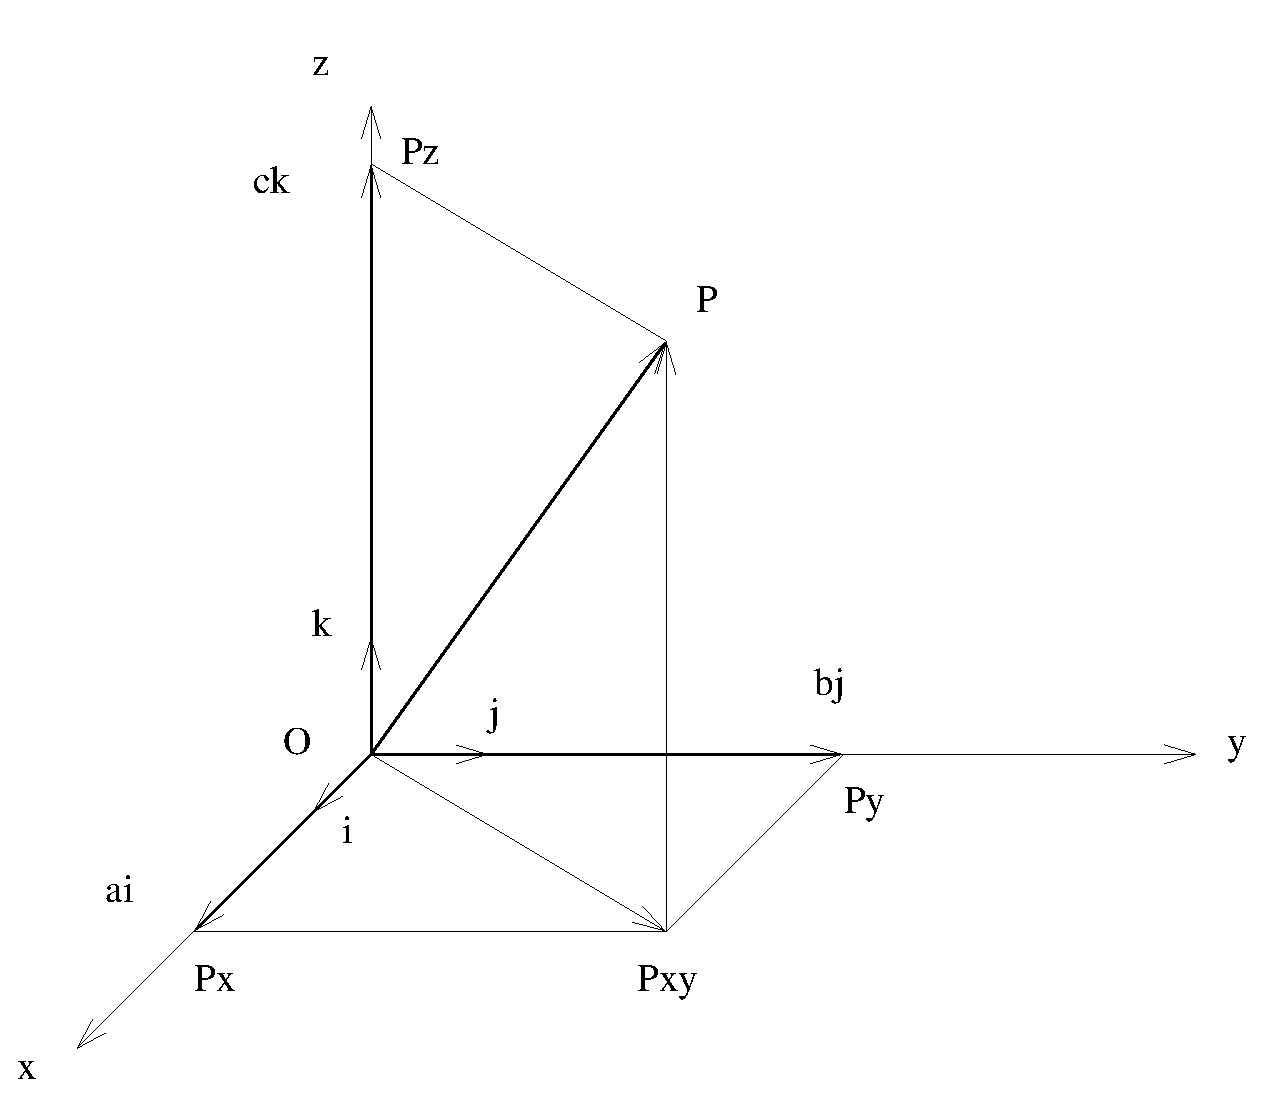
\includegraphics[height=2in]{../../modules/vectors/pictures/ok-vector_decomposition.eps}
  %\caption{Coordinates of a vector}
\end{figure}
%
$$\textbf{OP} = a\textbf{i}+b\textbf{j}+c\textbf{k} = \langle a, b, c\rangle\; .$$

\end{frame}
\begin{frame}
\frametitle{Operations in Coordinates}

\begin{itemize}
 \item Magnitude:
%
$$|\langle a, b, c \rangle| = |OP| = \sqrt{a^2+b^2+c^2}$$
%
\item Addition:
%
$$\langle x_1,y_1,z_1 \rangle + \langle x_2, y_2,z_2\rangle = \langle x_1+x_2, y_1+y_2, z_1+z_2\rangle\; .$$
%
\item Scalar multiple:
%
$$c\langle x, y, z\rangle = \langle cx, cy, cz\rangle\; .$$
%
\item General displacement from $A(x_A, y_A, z_A)$ to $B(x_B, y_B, z_B)$:
%
$$\textbf{AB} = \textbf{AO} +\textbf{OB} = \textbf{OB} - \textbf{OA} = \langle x_B-x_A, y_B-y_A, z_B-z_A\rangle \; .$$
\end{itemize}

\end{frame}